\documentclass[13pt,compress,c]{beamer}
\usepackage[brazil]{babel}
%\usepackage[latin1]{inputenc}
\usepackage[utf8]{inputenc}
\usepackage{listings}
\usepackage{latexsym}
\usepackage{amssymb}
\usepackage{graphicx}
\usepackage{relsize}          % for \smaller etc.


%\bibliographystyle{plain}

\setbeamercolor{normal text}{bg=blue!4}

%\usetheme{default}

% tema com vermelho
%\usetheme{CambridgeUS}

% tema com amarelo
%\usetheme{AnnArbor}

% tema azul
\usetheme{Boadilla}

% tema azul, aulas de mc348 e mc448
%\usetheme{Madrid}

% tema mais branco
%\usetheme{umbc1} 

\title[Códigos Corretores de Erros no HDFS]{Estudo e Implementação de Códigos Corretores de Erros no Sistema de Arquivos Distribuído do Hadoop}

\author[Celina d' Á. Samogin]{Celina d' Ávila Samogin\\
  Instituto de Computação --- UNICAMP}

\begin{document}

\frame{

   \begin{center}
     \large{Prévia da Defesa de Mestrado}
    \end{center}

    \titlepage

    \begin{center}
     Orientadora: Profa. Dra. Islene Calciolari Garcia
    \end{center}

}


% \section{Agenda}

\AtBeginSection[]
{
  \begin{frame}
   \frametitle{Agenda}
   \tableofcontents[currentsection]
  \end{frame}
}


 \frame{\tableofcontents}

\AtBeginSection[]
{
  \begin{frame}
   \frametitle{Agenda}
   \tableofcontents[currentsection]
  \end{frame}
}

  \section{Introdução}

  \begin{frame}{Motivação}
     \begin{itemize}
      \item Este trabalho é uma contribuição para \emph{software} livre em sistemas distribuídos.
      \item Armazenamento de dados $===>$ componente essencial na computação de alto desempenho. 
      \item Códigos Corretores de Erro (\emph{Erasure codes}) introduzem redundância para alcançar confiabilidade e redução do custo de armazenamento.    
     \end{itemize}
  \end{frame}

  \begin{frame}{Motivação}
   \begin{figure}[h]
     \centering
     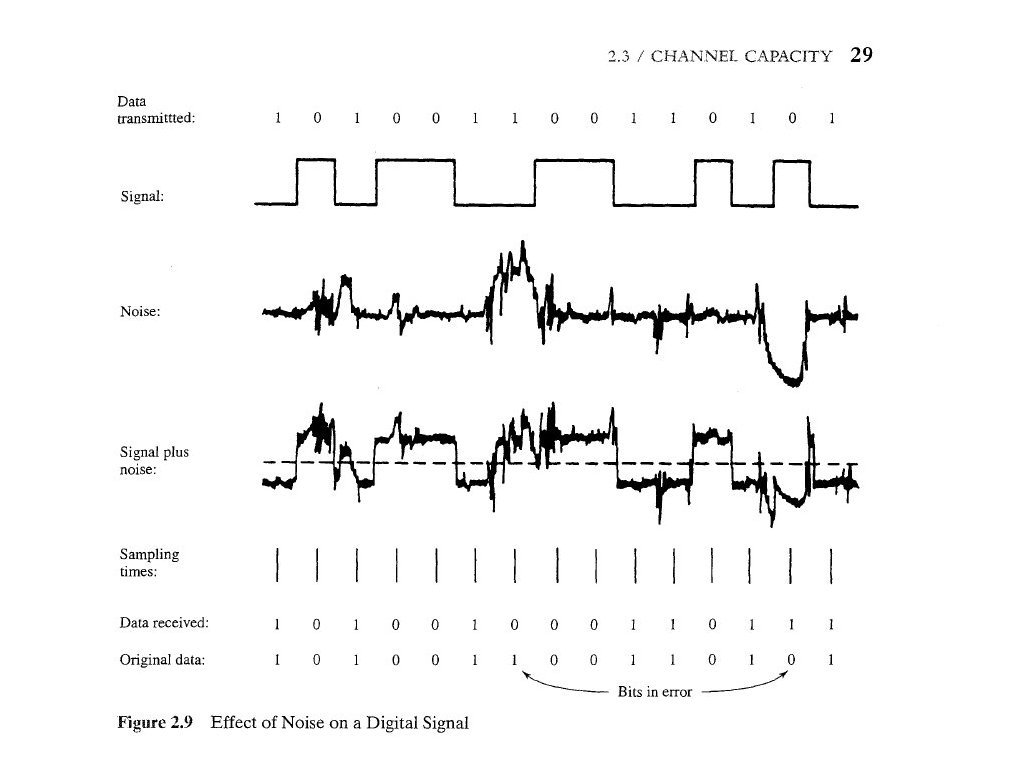
\includegraphics[scale=.25]{stalling-channel-capacity.jpg}
     \caption{Efeito do ruído no sinal digital \cite{Stallings:2005}}
     \label{fig1:ersd}
   \end{figure}
  \end{frame}

  \begin{frame}{Motivação}
     \begin{itemize}
         \item Popularização dos computadores e as pesquisas espaciais $==>$ os códigos corretores de erros tornaram-se parte comum de comunicações por satélite, de redes de computadores, de armazenamento em discos óticos e outros meios magnéticos.
         \item Uso frequente em nosso cotidiano
%quando se assiste a um programa de televisão, quando se ouve música a partir de um CD, quando se atende um telefonema, quando se assiste um filme gravado em DVD, quando se navega pela internet.
     \end{itemize}
  \end{frame}

% http://worldtelevisao.blogspot.com.br/2011/05/programas-infantis-que-fizeram-historia.html
  \begin{frame}{Motivação}
   \begin{figure}[h]
     \centering
     
\includegraphics[scale=.3]{enio-beto.jpg}
     \caption{Assistir programa de televisão Vila Sésamo\cite{WTPI:2012}}
     \label{fig7:tv}
   \end{figure}

% http://vidaanascer.blogspot.com.br/2012/09/notas-da-alma.html
   \begin{figure}[h]
     \centering
     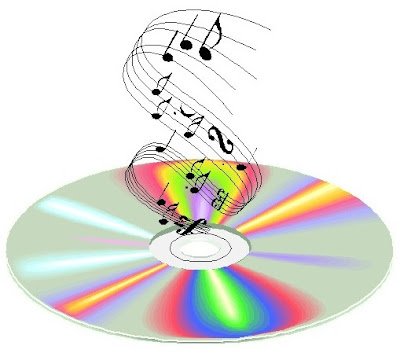
\includegraphics[scale=0.2]{music_cd.jpg}
     \caption{Ouvir música a partir de um CD\cite{MNA:2012}}
     \label{fig8:cd}
   \end{figure}
  \end{frame}

  \begin{frame}{Motivação}
% http://volneyf.blogspot.com.br/2008_04_01_archive.html
   \begin{figure}[h]
     \centering
     
\includegraphics[scale=0.3]{telephone-ringing.jpg}
     \caption{Atender um telefonema\cite{VF:2012}}
     \label{fig9:tel}
   \end{figure}


% http://phpbrasil.com/artigo/ozk4KmI6_tdC/2/criando-sites-para-celular-com-wml-parte-1
   \begin{figure}[h]
     \centering
     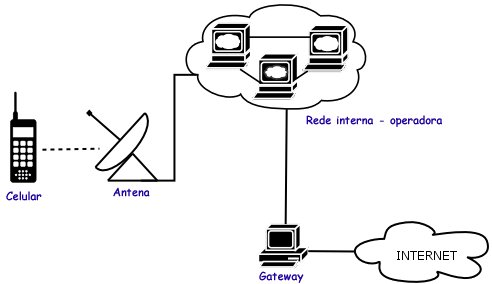
\includegraphics[scale=0.2]{internet-celular.jpg}
     \caption{Navegar pela internet\cite{FBP:2012}}
     \label{fig10:internet}
   \end{figure}
  \end{frame}

  \begin{frame}{Motivação}
     \begin{itemize}
      \item Alguns sistemas que utilizam códigos corretores de erros:
	\begin{itemize}
%           \item \emph{Digital Fountain} (\emph{multicasting} multimídia confiável)\cite{Byers:1998}
            \item \emph{NASA's Deep Space Network} no envio e na recepção de sinais e dados de telemetria
(\emph{downlinks}) vindos de veículos espaciais (\emph{very distant spacecrafts}) e para enviar telecomandos (\emph{uplinks}) para
% veículos espaciais \cite{Abrantes:2010, Almeida:2007, STO:2010, TDD:2010};
veículos espaciais;
%           \item \emph{Delay and Disruption Tolerant Networks}, redes de sensores e redes~\emph{peer-to-peer} \cite{Bhagwan:2004, Alencar:2004, Haeberlen:2005, Houri:2009,RTAD:2007, Rodrigues:2005, Wilcox-O'Hearn:2008};
           \item \emph{Delay and Disruption Tolerant Networks}, redes de sensores e redes~\emph{peer-to-peer};
%           \item armazenamento de grande volume de dados \cite{Anderson:1998,Kubiatowicz:2000,  Saito:2004, Schmuck:2002, Storer:2008,
% Storer:2009, Xia:2006}, como também o sistema de arquivos distribuído do Hadoop (HDFS)~\cite{HDFS-503:2010}.
           \item armazenamento de grande volume de dados, como também o sistema de arquivos distribuído do Hadoop (HDFS).
%           \item sistema de arquivos distribuído do Hadoop (HDFS)~\cite{HDFS-503:2010}
	\end{itemize}
     \end{itemize}
  \end{frame}

% http://www2.jpl.nasa.gov/basics/bsf10-1.php

%  \begin{frame}{Motivação}
%   \begin{figure}[h]
%     \centering
%     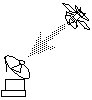
\includegraphics[scale=.3]{1-way.jpg}
%     \caption{1-\emph{way}: dados vindos de um veículo espacial\cite{Plank:2004}}
%     \label{fig2:1way}
%   \end{figure}
%   \begin{figure}[h]
%     \centering
%     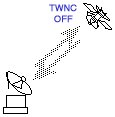
\includegraphics[scale=0.3]{2-way.jpg}
%     \caption{2-\emph{way}: dados vindos de um veículo espacial e comandos enviados para um veículo espacial\cite{Plank:2004}}
%     \label{fig3:2way}
%   \end{figure}
%   \begin{figure}[h]
%     \centering
%     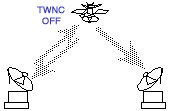
\includegraphics[scale=0.3]{3-way.jpg}
%     \caption{3-\emph{way}: dados vindos de dois veículos espaciais e comandos enviados para dois veículos espaciais\cite{Plank:2004}}
%     \label{fig4:3way}
%   \end{figure}
%  \end{frame}

% http://www.au.af.mil/au/awc/awcgate/jplbasic/bsf10-1.htm
% Two-Way Non-Coherent

  \begin{frame}{Motivação}
   \begin{figure}[h]
     \centering
     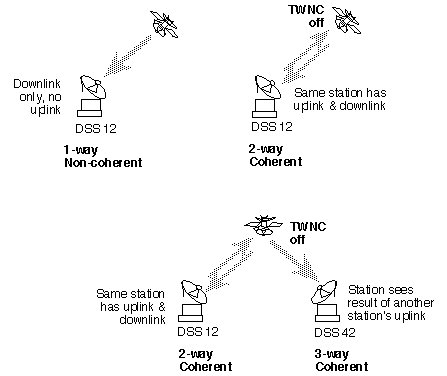
\includegraphics[scale=.4]{bsfii6.jpg}
     \caption{\emph{NASA's Deep Space Network}\cite{JPLCIT:2012}}
     \label{fig2:nasa}
   \end{figure}
  \end{frame}

% Venturebeat.com/2012/11/14/facebook-north-carolina-data-center/
  \begin{frame}{Motivação}
   \begin{figure}[h]
     \centering
     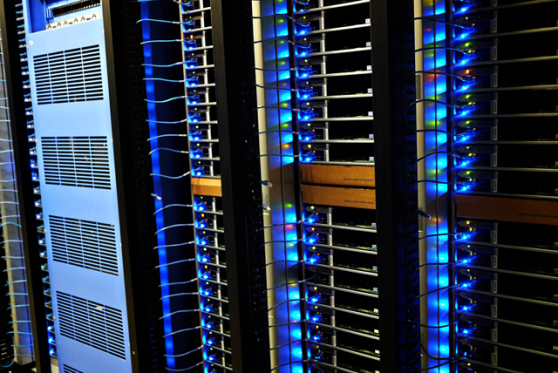
\includegraphics[scale=.5]{facebook-data-center.jpg}
     \caption{Facebook data center\cite{VBFB:2012}}
     \label{fig5:fdc}
   \end{figure}
  \end{frame}

  \begin{frame}{Motivação}
     \begin{itemize}
      \item O HDFS, por padrão, implementa alta disponibilidade dos dados via replicação simples dos blocos de dados. Esta abordagem acarreta um alto custo de armazenamento para garantir que os dados estarão sempre disponíveis.
      \item Esforços iniciais $===>$ \emph{Redundant Array of Independent Drives} (RAID)~\cite{HDFS-503:2010,Patterson:1988} e mais recentemente, Reed-Solomon (RS)~\cite{MR-1969:2010}.
     \end{itemize}
  \end{frame}


  \begin{frame}{Motivação}
     \begin{itemize}
        \item RAID (\emph{Redundant Arrays of Inexpensive [Independent] Disks} (RAID), do ponto de vista de suas estruturas algébricas, é uma classe de códigos de blocos lineares.
        \item RAID é um método para prover tolerância a falhas ou alto desempenho em sistemas de armazenagem utilizando, para isso, distribuição de dados em diferentes dispositivos e uma codificação de correção de erros ou paridade ou replicação de dados~\cite{Ramakrishnan:2003}.
        \item RAID foi introduzido por D. A. Patterson na Universidade da California, Berkeley (UC Berkeley) em 1988 \cite{Patterson:1988}.
        \item O código fonte do Hadoop implementa RAID-5, que na sua versão clássica, "fatia" dados e paridade, através dos discos, como num arranjo. A única paridade é calculada através da operação \emph{bitwise} XOR. 
     \end{itemize}
  \end{frame}

% \footnote{Essa definição foi apresentada pelo Prof.dr.ir Henk C.A. Van Tilborg, pesquisador da Technische Universiteit Eindhoven, na sua palestra Old and New(er) Results in the Theory of Burst-Correcting Codes em 23 de novembro no Instituto de Matemática, Estatística e Computação Científica da Universidade Estadual de Campinas.}

 \begin{frame}{Motivação}
    \begin{figure}[hb]
      \centering
      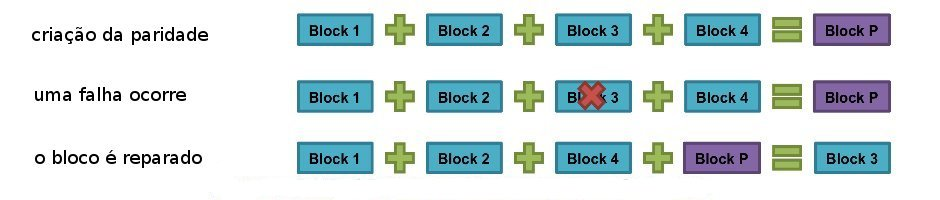
\includegraphics[scale=0.35]{raid5.jpg}
      \caption{RAID 5: 1 bloco de paridade e \emph{stripe} = 4 blocos \cite{MR-2036:2010}}
      \label{fig5:raid5}
    \end{figure}
 \end{frame}


  \begin{frame}{Motivação}
     \begin{itemize}
        \item Códigos Reed-Solomon (RS) são códigos de bloco, lineares e cíclicos (sobre anéis comutativos sob algumas condições).
        \item Parametrizáveis $===>$ capacidade de correção de erros pode ser alterada facilmente.
        \item RS são códigos MDS $===>$ as palavras-código apresentam máxima distância de Hamming entre si, permitida pelo número de dígitos de verificação de paridade do código.
        \item Segundo os autores em \cite{Almeida:2007,Sloane:1977}, códigos RS são úteis para correção de erros em rajada.
\begin{definition} {\bf Burst Errors} \index{Burst Errors} Uma sequência de erros em rajada ou \emph{burst errors} de tamanho $b$ é da forma:
    \begin{align*}
     (0, 0, \ldots, 0, 1, \ldots , 1, 0, \ldots, 0, 0)
    \end{align*}
onde o primeiro bit $1$ está na $i$-posição e o último bit $1$ está na $(i+b-1)$-posição e entre esses primeiro e último bits existe uma sequência de $b$ bits quaisquer.
\end{definition}
     \end{itemize}
  \end{frame}

% http://pic.dhe.ibm.com/infocenter/powersys/v3r1m5/index.jsp?topic=/arebk/raidsix.htm
  \begin{frame}{Motivação}
   \begin{figure}[h]
     \centering
     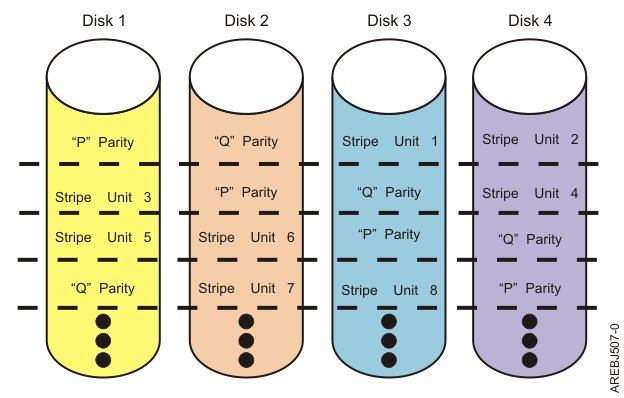
\includegraphics[scale=.4]{raid6.jpg}
     \caption{RAID 6 clássico "fatia" dados e paridade, através dos discos, como num arranjo. A paridade P e Q são geradas pela operação \emph{bitwise} XOR e pelo algoritmo Reed-Solomon.\cite{IBMR6:2012}}
     \label{fig6:raid6}
   \end{figure}
  \end{frame}

  \begin{frame}{Objetivos deste trabalho}

  \begin{itemize}
     \item avaliação de desempenho, ganhos, e custos de diferentes
  estratégias de códigos corretores de erro;
     \item implementação de otimizações ou extensões para o código fonte que
  atualmente implementa Reed-Solomon, tentando melhorar,
  principalmente, a parte de distribuição de blocos;
     \item implementação de novos algoritmos (Tornado e Turbo \emph{codes}) e
  extensão da interface atual para aceitá-los;
     \item integração do código fonte atual com o HDFS.
     \end{itemize}
  \end{frame}


  \section{Contexto em Sistemas Distribuídos e em Software Livre}

  \begin{frame}{Sistemas de Arquivos Distribuídos}
     \begin{itemize}
      \item<1-> Processar um volume relativamente grande de dados é possível, em poucas horas, com alguns dólares e com algumas máquinas: http://aws.amazon.com/
      \item<2-> Isto também pode ser feito com o Hadoop, um \emph{framework} para processamento de dados em larga escala.
      \item<3-> Volume grande de dados ?
          \begin{itemize}
             \item<4-> megabyte - $10^6$ - uma foto
             \item<5-> gigabyte - $10^9$ - um DVD armazena 4.7 GB de um filme
             \item<6-> terabyte - $10^{12}$ - 200 filmes
             \item<7-> petabyte - $10^{15}$
             \item<8-> exabyte - $10^{18}$
             \item<9-> zettabyte - $10^{21}$ - um disco de 140 GB para cada pessoa no mundo
          \end{itemize}
     \end{itemize}
  \end{frame}

  \begin{frame}{Software Open Source}

% http://feedgrowth.com/idea-categories/social-networking/secure-your-brands-username-and-vanity-url-on-facebook/
   \begin{figure}[hb]
     \centering
     
\includegraphics[scale=0.3]{facebook-logo.jpg}
     
\includegraphics[scale=0.2]{yahoo-logo-300x224.jpg}
     
\includegraphics[scale=1]{google-logo.jpg}
     
\includegraphics[scale=0.06]{new-twitter-logo.jpg}
     
\includegraphics[scale=0.1]{lastfm.jpg}
     
\includegraphics[scale=0.1]{microsoft-logo.jpg}
     
\includegraphics[scale=0.1]{IBM-logo.jpg}
%     \caption{Facebook www.facebook.com}
     \label{fig11:fb}
   \end{figure}

% http://www.scienceweek.ie/features/2012-featured-articles/google-experiments.html
%   \begin{figure}[hb]
%     \centering
%     
\includegraphics[scale=1]{google-logo.jpg}
%     \caption{Facebook www.facebook.com}
%     \label{fig12:goo}
%   \end{figure}

% http://theinspirationroom.com/daily/2012/twitter-logo-redesigned/
%   \begin{figure}[hb]
%     \centering
%     
\includegraphics[scale=0.1]{new-twitter-logo.jpg}
%     \caption{Facebook www.facebook.com}
%     \label{fig13:twi}
%   \end{figure}

% http://www.telegraph.co.uk/technology/microsoft/9495544/Microsoft-unveils-new-logo.html
%   \begin{figure}[hb]
%     \centering
%     
\includegraphics[scale=0.2]{microsoft-logo.jpg}
%     \caption{Facebook www.facebook.com}
%     \label{fig14:ms}
%   \end{figure}

% http://darts.cse.nd.edu/projects/ibm-logo/
%   \begin{figure}[hb]
%     \centering
%     
\includegraphics[scale=0.1]{IBM-logo.jpg}
%     \caption{Facebook www.facebook.com}
%     \label{fig15:ibm}
%   \end{figure}


% http://www.cloudbook.net/directories/research-clouds/university-of-maryland-college-park
% http://creeva.com/2012/03/08/i-have-successfully-merged-last-fm-accounts-here-is-a-howto/
% http://terrierteam.dcs.gla.ac.uk/

   \begin{figure}[hb]
     \centering
     
\includegraphics[scale=1]{CompScience_colour_stk-2.jpg}
     
\includegraphics[scale=0.3]{university_of_maryland_college_park_logo2.jpg}
     
\includegraphics[scale=0.3]{cornell.jpg}
%     \caption{Facebook www.facebook.com}
     \label{fig11:fb}
   \end{figure}

% http://tomcat.apache.org/
   \begin{figure}[hb]
     \centering
     
\includegraphics[scale=0.2]{asf-logo.jpg}
      
\includegraphics[scale=2]{hadoop-logo.jpg}
%     \caption{Facebook www.facebook.com}
     \label{fig16:afs}
   \end{figure}

     \begin{itemize}
        \item<1-> O Hadoop disponibiliza um armazenamento compartilhado (HDFS/Hadoop \emph{Distributed Filesystem}) e um sistema de análise (MapReduce), formando um \emph{framework} ou arcabouço.
%         \item<2-> Facebook, Google, Twitter, Microsoft e IBM armazenam dados do tamanho de petabytes e utilizam o Hadoop.
%         \item<3-> O projeto Hadoop é hoje um projeto independente dentro da hierarquia de projetos da Apache Software Foundation.
     \end{itemize}
  \end{frame}

  \begin{frame}{RDBMS X HDFS/MapReduce}
    Por que não usamos banco de dados ?
     \begin{itemize}
        \item<1->  Em um banco de dados, uma atualização da árvore-B pode gerar muitas operações de \emph{seeking}.
        \item<2->  \emph{seek time} - processo de mover a cabeça do disco para um dado local no disco com o objetivo de ler ou de escrever dados
        \item<3->  É mais rápido usar um algoritmo de ordenação (\emph{sort}/\emph{merge}) para:
          \begin{itemize}
             \item<4-> analisar um grande volume de dados do tamanho de petabytes
             \item<5-> reconstruir toda a base de dados
          \end{itemize}
      \end{itemize}
  \end{frame}

  \begin{frame}{RDBMS X HDFS/MapReduce}
{\small
        \begin{center}
          \begin{tabular}{|p{2cm}||p{3.5cm}||p{3.5cm}|}
            \hline
& Aplicação para RDBMS & Aplicação para HDFS/MapReduce\\ \hline
tamanho & gigabytes & petabytes\\ \hline
acesso & OLTP(interativo) e \emph{batch} & \emph{batch}\\ \hline
atualização & lê e escreve muitas vezes & escreve uma vez, lê muitas vezes\\ \hline
esquema & estático & dinâmico\\ \hline
integridade & alta & baixa\\ \hline
escala & não linear & linear\\ \hline
          \end{tabular}
        \end{center}
}

Fonte: \cite{White:2009}
  \end{frame}

  \begin{frame}{HDFS}

    \begin{figure}[hb]
      \centering
      
\includegraphics[scale=2]{hadoop-logo.jpg}
%      \caption{Projeto Hadoop \cite{Hadoop:2010}}
%      \label{fig5:php}
    \end{figure}

HFS disponibiliza espaço para sistema de arquivos e permite que os dados do usuário sejam armazenados em arquivos. Internamente, um arquivo é dividido em um ou mais blocos e esses blocos são armazenados em um conjunto de DataNodes. O tamanho \emph{default} de cada bloco é 64MB.

    \begin{figure}[hb]
      \centering
      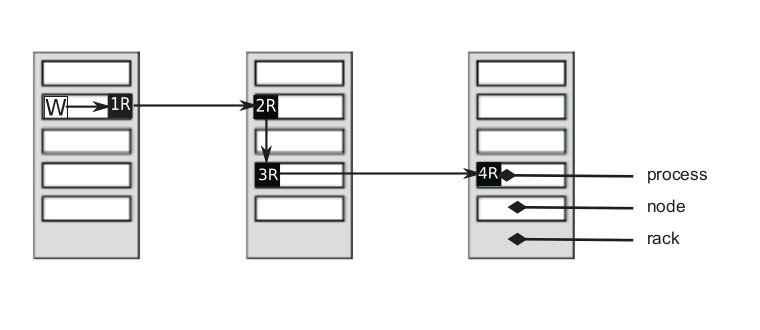
\includegraphics[scale=0.4]{HDFS-arquitetura-replicacao-2.jpg}
      \caption{Arquitetura do HFS - Datanodes e Blocos \cite{Hadoop:2010}}
      \label{fig7:hfs}
    \end{figure} 

  \end{frame}


  \begin{frame}{MapReduce}

    \begin{figure}[hb]
      \centering
      
\includegraphics[scale=2]{hadoop-logo.jpg}
%      \caption{Projeto Hadoop \cite{Hadoop:2010}}
%      \label{fig5:php}
    \end{figure}

     \begin{itemize}
       \item<1-> Os dados que MapReduce processa são dados não estruturados como texto ou imagens. O HDFS, através do \emph{pipeline} dos DataNodes, tenta colocar esses dados no nó onde são feitas as computações, desta forma, o acesso aos dados é rápido, pois é "mais" local.
       \item<2-> O MapReduce pode resolver problemas genéricos cujos dados podem ser divididos em matrizes de dados, para cada matriz a mesma computação é necessária e não existe necessidade de comunicação entre as tarefas.
       \item<3-> Problemas como empacotamento, linha de fábrica, otimização não são resolvidos pelo modelo de computação do MapReduce.
     \end{itemize}

  \end{frame}

  \begin{frame}{MapReduce}

    \begin{figure}[hb]
      \centering
      
\includegraphics[scale=2]{hadoop-logo.jpg}
%      \caption{Projeto Hadoop \cite{Hadoop:2010}}
%      \label{fig5:php}
    \end{figure}

Problema genérico:
\begin{itemize}
   \item iteração sobre um número grande de registros
   \item \emph{Map} extrai algo de cada registro (chave, valor)
   \item rearranjo (\emph{shuffle} e ordenação de resultados intermediários por (chave, valor)
   \item \emph{Reduce} agrega os resultados intermediários 
   \item geração da saída
\end{itemize}

  \end{frame}



  \section{Métodos utilizados nesse Estudo e nessa Implementação}

  \begin{frame}{Álgebra Abstrata e de Códigos Corretores de Erros}
     \begin{itemize}
        \item<1-> \emph{Erasure Coding}
        \item<2-> Exame de Qualificação para o Mestrado (EQM)
        \item<3-> Foco: armazenamento de dados
        \item<4-> Códigos corretores de erro disponíveis na versão 0.22  do Hadoop: RAID e RS
    \begin{figure}[hb]
      \centering
      
\includegraphics[scale=2]{hadoop-logo.jpg}
%      \caption{Projeto Hadoop \cite{Hadoop:2010}}
%      \label{fig5:php}
    \end{figure}

        \item<5-> Muitos artigos e material de aulas das disciplinas de universidades de Portugal, Índia, Paquistão e EUA

     \end{itemize}
  \end{frame}

  \begin{frame}{Intuições na Álgebra Abstrata}
     \begin{itemize}
        \item<1-> Congruência linear
        \item<2-> Classes Residuais
        \item<3-> Resto da divisão euclidiana
        \item<4-> Independência linear
        \item<5-> Espaço Vetorial, Grupo, Anel e Corpo (principalmente $\mathbb{GF}_2$ e $\mathbb{GF}_{256}$)
        \item<6-> Sistema de Equações Lineares
        \item<7-> Matrizes
        \item<8-> Polinômios
     \end{itemize}
  \end{frame}

\begin{frame}{Intuições na Álgebra Abstrata}
\begin{definition} {\bf Congruência Linear} \index{Congruência Linear} Seja $q \in \mathbb{Z}$. Dois inteiros $a$
 e $b$ dizem-se congruentes módulo $q$ se, e somente se, $q$ divide $a - b$. A notação é $a \equiv b\,(mod\ q)$. Assim, $a - b\ \in$ $\{x\ tal\ que\ x =  kq, k \in \mathbb{Z}\}$.
\end{definition}

\begin{example}
\begin{align*} % Dois environments aninhados; precisamos arrumar o excesso de espaçamento.
& 32 \equiv 2\,(mod\ 3)\\
& 27 \equiv 5\,(mod\ 11)\\
& 63 \equiv 7\,(mod\ 8)
\end{align*}
\end{example}
  \end{frame}

\begin{frame}{Intuições na Álgebra Abstrata}
\begin{definition} {\bf Conjunto das Classes Residuais} \index{Conjunto das Classes Residuais} Seja $\mathbb{Z}/q = \{\bar{0}_q, \bar{1}_q, \ldots , \overline{q-1}_q\}$ o conjunto das classes residuais dos inteiros módulo $q$. 
\end{definition}

Note que $\mathbb{Z}/q$ tem exatamente $q$ elementos, portanto $\mathbb{Z}/q$ é finito.

As classes residuais possuem propriedades:
  \begin{enumerate}[(i)]
      \item Se a$\ \equiv\ b\,(mod\ q)$, então $\bar{a}_q = \bar{b}_q$.
      \item Se $\bar{a}_q \cap \bar{b}_q  \neq 0$, então $\bar{a}_q = \bar{b}_q$.
      \item Para $a \in \mathbb{Z}, \bigcup \bar{a}_q = \mathbb{Z}$.
  \end{enumerate}

  \end{frame}

  \begin{frame}{Conceitos em Códigos Corretores de Erros}
     \begin{itemize}
        \item<1-> Teoria da codificação $===>$ propriedades dos códigos e suas aplicações
        \item<2-> Teoria da Informação, Claude Shannon~\cite{Shannon:1948} $===>$ incerteza da informação e capacidade do canal
        \item<3-> C. Shannon estudou o processamento digital de sinais (sinais em tempo discreto e em tempo contínuo) em um sistema de comunicação $===>$ hoje, é área da engenharia elétrica e da matemática aplicada
        \item<4-> Sinais podem ser som, áudio, dados biológicos como eletrocardiogramas ou sequências de DNA~\cite{Faria:2010,Faria:2012}, sinais de sistemas de telecomunicações, entre muitos outros.
        \item<5-> Objetivo da codificação de canal é aumentar a resistência do sistema de comunicações digital face aos efeitos do ruído de canal.
     \end{itemize}
  \end{frame}

  \begin{frame}{Conceitos em Códigos Corretores de Erros}
     \begin{itemize}
        \item<1-> Canal binário simétrico
    \begin{figure}[hb]
      \centering
      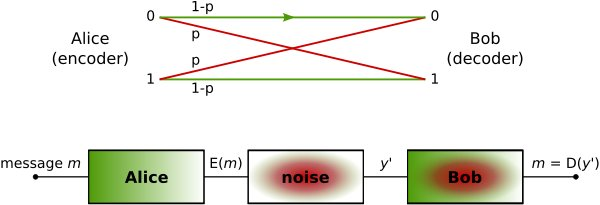
\includegraphics[scale=0.5]{600px-Binary_symmetric_channel.jpg}
%      \caption{Projeto Hadoop \cite{Hadoop:2010}}
%      \label{fig5:php}
    \end{figure}
     \end{itemize}
  \end{frame}

  \begin{frame}{Conceitos em Códigos Corretores de Erros}
     \begin{itemize}
        \item<1-> A ciclicidade de códigos sob anéis comutativos está associada à multiplicação do polinômio gerador pelos diferentes potências de "x" reduzida módulo um polinômio irredutível.
     \end{itemize}
  \end{frame}

  \begin{frame}{Conceitos em Códigos Corretores de Erros}
     \begin{itemize}
        \item<1-> Detectar erros e codificar dados tem a mesma complexidade 
        \item<2-> Decodificar é np-completo
        \item<3-> Estruturas algébricas: matrizes
     \end{itemize}
  \end{frame}

  \begin{frame}{Conhecer e Compilar o código fonte disponível}
   \begin{figure}[hb]
     \centering
     
\includegraphics[scale=0.3]{facebook-logo.jpg}
     
\includegraphics[scale=0.2]{yahoo-logo-300x224.jpg}
     
\includegraphics[scale=0.2]{asf-logo.jpg}
%     \caption{Facebook www.facebook.com}
     \label{fig11:fb}
   \end{figure}
     \begin{itemize}
        \item<1-> Facebook, Yahoo, Fundação Apache
        \item<2-> O \emph{kernel} do Hadoop é constituído do core, hdfs e mapred.
        \item<3-> As versões oficiais para instalação (http://www.apache.org/dist/hadoop/core/) e
        \item<4-> as versões do código fonte (common, hdfs, mapreduce) estão disponíveis em repositório SVN (https://svn.apache.org/repos/asf/hadoop/common/branches/branch-0.22) 
        \item<5-> Na atividade \emph{Scripts for building Hadoop 0.22.0 release}  https://issues.apache.org/jira/browse/HADOOP-6846, os mantenedores e contribuidores do Hadoop discutiam como compilar a versão 0.22
     \end{itemize}
  \end{frame}

  \begin{frame}{Conhecer e Compilar o código fonte disponível}
     \begin{itemize}
        \item<1-> Eclipse IDE for Java
        \item<2-> comandos do linux, principalmente, grep, find e editores de texto
        \item<3-> Doxygen para gerar diagramas de herança e de colaboração das classes a partir do código fonte
        \item<4-> Implementar uma aplicação do \emph{framework} do Hadoop: conta-palavras, temperatura máxima, \emph{page rank}
        \item<5-> Fazer uma pequena alteração no código fonte do RaidNode () para escrever uma mensagem no arquivo de log, compilar o código fonte modificado, instalá-lo e testá-lo
     \end{itemize}
  \end{frame}

  \begin{frame}{Conhecer e Compilar o código fonte disponível}
     \begin{itemize}
        \item<1-> Hadoop foi escrito quase que inteiramente em Java: construtores de classe, asserções
        \item<2-> Java: 1o capítulo do livro vermelho do Sedgewick, Algorithms
        \item<3-> Entender a camada RAID para poder extendê-la
        \item<4-> Entender de álgebra abstrata e de uma de suas aplicações: códigos corretores de erros
        \item<5-> Propor os algoritmos dos novos \emph{codecs}: \emph{encode} e \emph{decode}
     \end{itemize}
  \end{frame}

  \begin{frame}{Conhecer e Compilar o código fonte disponível}
     \begin{itemize}
        \item<1-> Ambiente de edição do código fonte das classes
           \begin{itemize}
              \item<2-> Notebook com Ubuntu $8.04$, depois $10.04$, depois $12.04$ ($2GB$ de RAM, \emph{dual-core}, $150MB$ de disco interno, $1.35TB$ de disco externo) 
           \end{itemize}
        \item<3-> Ambiente de compilação do Hadoop versão 0.22
           \begin{itemize}
              \item<4-> Notebook com Ubuntu
              \item<5-> Laboratório da pós-graduação do IC; estação $64$ bits com Fedora
              \item<6-> Instâncias da Amazon EC2 (servidoras virtuais na Nuvem) com Ubuntu $12.10$,  \emph{kernel},  ($613MB$ de RAM, \emph{dual-core}, alguns \emph{gigabytes} de disco)
           \end{itemize}
        \item<7-> Ambiente de instalação do \emph{tarball}
           \begin{itemize}
              \item<8-> Notebook com Ubuntu
              \item<9-> Instâncias da Amazon EC2
           \end{itemize}
     \end{itemize}
  \end{frame}

  \begin{frame}{Testes Iniciais}
     \begin{itemize}
        \item<1-> Notebook com Ubuntu
        \item<2-> Testes funcionais: \emph{encode} e \emph{decode} das novas codificações e correção de erros no código fonte das classes das codificações implementadas por esse trabalho $===>$ linguagem Java.
     \end{itemize}
  \end{frame}

  \begin{frame}{Testes Finais}

     \begin{itemize}
        \item<1-> Instâncias da Amazon EC2 (servidoras virtuais na Nuvem) com Ubuntu $12.10$,  \emph{kernel},  ($613MB$ de RAM, \emph{dual-core}, alguns \emph{gigabytes} de disco)
        \item<2-> AWS Console e Amazon EC2 API tools (ferramentas de linha de comando)
        \item<3-> 3 fases de Testes de Desempenho (coleta de dados) da operação de \emph{encode} e de Injeção de Falhas das operações de \emph{encode} e \emph{decode} das novas codificações
        \item<4-> Primeira fase: preparação do ambiente de teste
        \item<5-> Rede de 4 instâncias: 1 \emph{master/slave} e 3 \emph{slaves}
        \item<6-> Base de dados: imagens ISO  ($+-800MB$ cada uma)
     \end{itemize}
  \end{frame}

  \begin{frame}{Testes Finais}
     \begin{itemize}
        \item<1-> Segunda fase: coleta de dados para medição de desempenho da operações de \emph{encode} e de \emph{decode} para cada codificação:
                  \begin{itemize}
                     \item replicação simples $2X$
                     \item replicação simples $3X$
                     \item $XOR(6,5)$
                     \item $RS(8,5)$
                     \item $Tornado(10,5)$
                     \item $Tornado(20,10)$
                     \item $Turbo-like(10,5)$
                     \item $Turbo-like(20,10)$
                 \end{itemize}
              \item<2-> Rede de 16 instâncias \emph{large}, provavelmente
        \item<2-> Base de dados: imagens ISO
     \end{itemize}
  \end{frame}

  \begin{frame}{Testes Finais}
     \begin{itemize}
        \item<1-> Terceira fase: coleta de dados para medição da injeção de falhas
           \begin{description}
              \item [falha em $1$ réplica]: corromper $1$ réplica de blocos de dados de um arquivo
              \item [falha em $n$ réplicas] corromper $n$ réplicas de blocos de dados de um arquivo
              \item [falha em réplicas e em blocos de dados] corromper $n$ réplicas de blocos de dados e os $k-1$ blocos de dados de um arquivo
            \end{description}
        \item<2-> Rede de 16 instâncias \emph{large}, provavelmente
        \item<3-> Base de dados: imagens ISO
     \end{itemize}
  \end{frame}

  \begin{frame}{Testes Finais}

     \begin{table}
%\singlespacing
%{\footnotesize
{\scriptsize
    \centerline{
    \begin{tabular}{ll}
       Métricas por Codificação & Origem\\ \hline
       Tempo total de execução do experimento & sistema operacional\\
       Tamanho do arquivo carregado no hdfs & interface web do hdfs\\
       Tempo de carga no hdfs por arquivo & arquivo de log do RaidNode\\
       Tempo de execução/encode por arquivo codificado & arquivo de log do RaidNode\\
       Tempo de execução/decode por arquivo decodificado & arquivo de log do RaidNode\\
       Número de iterações na execução do decode & arquivo de log do RaidNode\\
       Tamanho do bloco do hdfs & arquivo de configuração do hdfs\\
       Número de blocos da \emph{stripe} & arquivo de configuração do hdfs\\
       Fator de redundância previsto por arquivo & texto desta dissertação\\
       Fator de redundância por arquivo obtido nos experimentos & interface web do hdfs\\
       Número de blocos com falhas suportado & arquivo de configuração do hdfs\\
       Número de blocos com falhas obtido nos experimentos & arquivo de log do RaidNode\\
    \end{tabular}}
    \caption{Métricas quantitativas coletadas por codificação nos experimentos para operações de \emph{encode} e de \emph{decode}}
    \label{tab10:metri}
}
\end{table}


  \end{frame}


%  \section{Algoritmos}


 \section{Resultados}

\begin{frame}{Resultados}

   \begin{itemize}

      \item Esse trabalho estendeu e alterou código fonte distribuído sob a licença Apache. 

      \item Com as codificações RAID, RS, já disponíveis no HDFS e as codificações Tornado e Turbo-like, implementadas por esse trabalho de mestrado, o HDFS disponibiliza, com uma flexível configuração, as principais codificações para canal binário simétrico
%, ou seja, códigos lineares, sendo que, o único código cíclico é RS. RAID, Tornado e Turbo-\emph{like} são códigos que são um sub-conjunto de códigos LDPC, que são códigos baseados em grafos regulares e em grafos irregulares.

      \item Os diagramas de herança e de colaboração para as classes, o código dos procedimentos de compilação e de geração do arquivo \emph{tarball} e o código da implementação das codificações foram disponibilizados em repositório público \footnote{https://github.com/celinasam/}.

  \end{itemize}

\end{frame}

\begin{frame}{Resultados}

   \begin{itemize}

      \item Foram criados um site \footnote{https://sites.google.com/site/newerasurecodinginhadoop} com comentários dos resultados obtidos desse trabalho e um \emph{blog} \footnote{http://mcss.posterous.com/} para comentar assuntos que a autora considerou de grande interesse para outras pessoas.

      \item Um dos cenários de uso de codificações baseadas em grafos seria em ambientes de \emph{data center}, onde um grande número de máquinas poderiam falhar. Com blocos de paridade íntegros dos arquivos com, pelo menos, 1 dos blocos de dados dos mesmos arquivos disponível, há uma grande probabilidade desse tipo de codificação recuperar os blocos de dados corrompidos. Essa é uma aplicação das codificações implementadas por esse trabalho.
  \end{itemize}

\end{frame}

\begin{frame}{Trabalhos Futuros}

   \begin{itemize}

      \item Esse trabalho discutiu esquemas adequados de redundância de dados apenas sobre o aspecto do esquema de dados, sem comentar algoritmos de atualização das réplicas. O teorema da Codificação do Canal~\cite{Abrantes:2010,Schwartz:1990} afirma que um sistema com largura de banda a maior possível tem uma capacidade de canal finita. Em esboços preliminares, comparando-se, para uma dada codificação, pode-se concluir que a probabilidade de erro em uma palavra código sem codificação é maior que a probabilidade de erro em uma palavra código com codificação.

       \item O estudo da independência das réplicas de um esquema de redundância é um campo promissor para pesquisas. A avaliação de esquemas de redundância é muitas vezes baseada na suposição de que as réplicas falham de forma independente. Na prática, as falhas não são tão independentes, segundo \cite{Weatherspoon:2002:02,Baker:2006}.

%        \item A construção de novas codificações, aplicando técnicas como as apresentadas no \emph{paper} de Andrade, Shan e Khan~\cite{Andrade:2011} apresenta algumas implicações, o que provavelmente, nesse caso, significa alterações no micro-código da linguagem assembler de uma plataforma software e também uma possível redução no número de operações para codificar e/ou decodificar em detrimento do aumento do tamanho do armazenamento de dados.

  \end{itemize}

\end{frame}

\begin{frame}{Trabalhos Futuros}
   \begin{itemize}

        \item Uma extensão do algoritmo da camada RAID pode melhorar o desempenho da tolerância à falhas.
%, pois RAID demonstra ser a codificação mais simples de se implementar que outras que exigem um projeto muito sofisticado do decodificador.

        \item Aplicações de códigos corretores de erros em outros canais binários simétricos e suas extensões como \emph{joint source–channel coding} parecem uma pesquisa promissora, pois "contenar" codificação de fonte e de canal, tem sido proposto para implementar aplicações que tem requisitos de tempo-real como transmissão de áudio e imagem em um canal binário simétrico com ruído~\cite{JSCC:2012}.

        \item O estudo e a implementação de outros mecanismos e técnicas para redução de armazenamento e disponibilidade de dados, otimizando o desempenho de codificações baseadas em grafos, como códigos LDPC
%, também é um desafio, visto que, o número de operações para codificar e/ou decodificar pode ser maior com essas codificações do que com outras, como códigos cíclicos, cujo projeto do decodificador é mais complexo.

        \item O estudo e implementação de aplicações de códigos corretores de erros, tanto a com memória como a sem memória, para os canais do DNA e do RNA~\cite{Rocha:2010,Faria:2012} é uma pesquisa bastante desafiadora e promissora.

  \end{itemize}

\end{frame}

 \begin{frame}{Interação com a comunidade}
   \begin{itemize}
      \item As versões do hadoop relacionadas a esta proposta: 0.20.1, 0.21.0 e 0.22.0 do Hadoop
      \item Analisadas um pouco mais de 120 discussões do jira
      \item Buscas no jira issues.apache.org/, selecionando projeto "Hadoop Map/Reduce" e componente "contrib/raid", mostram algumas discussões sobre as camadas de codificação por apagamento
      \item camada RAID: versão 0.21.0 (discussão HDFS-503)
      \item codificação RS: versão 0.22.0 (discussões MAPREDUCE-1969 e MAPREDUCE-1970)
      \item codificação Tornado e Turbo-\emph{like}: possivelmente em versões futuras
   \end{itemize}
 \end{frame}

 \begin{frame}{Interação com a comunidade}
   \begin{itemize}
      \item Existe um grupo de contribuidores (de várias empresas como Cloudera, Facebook, Yahoo e de universidades como \emph{University of} Waterloo e Carnegie Mellow \emph{University}) da camada RAID, dos quais, destacamos Rodrigo Schmidt, ex-aluno do programa de pós-graduação deste Instituto, que sugeriu o tema deste trabalho e que tem contribuído com várias idéias para a realização deste trabalho.
      \item Esperamos interação e colaboração com os desenvolvedores.
   \end{itemize}
 \end{frame}

\begin{frame}{Agradecimentos}

   \begin{itemize}
        \item CNPq (Conselho Nacional de Desenvolvimento Científico e Tecnológico)
        \item FAPESP (Fundação de Amparo à Pesquisa do Estado de São Paulo)
        \item IC (Instituto de Computação da Unicamp)
        \item Embrapa (Empresa Brasileira de Pesquisa Agropecuária)
  \end{itemize}

\end{frame}


\section{Referências Bibliográficas}

\begin{frame}[allowframebreaks,allowdisplaybreaks]{Referências Bibliográficas}

%  \smaller[5]

  \bibliographystyle{plain}
%  \setbeamertemplate{bibliography item}[book] 
  \bibliography{apresentacao}

\end{frame}



\end{document}
